\chapter{Chương 3}
\ifpdf
    \graphicspath{{Chapter3/Chapter3Figs/PNG/}{Chapter3/Chapter3Figs/PDF/}{Chapter3/Chapter3Figs/}}
\else
    \graphicspath{{Chapter3/Chapter3Figs/EPS/}{Chapter3/Chapter3Figs/}}
\fi

\section{First Section of the Third Chapter}
\markboth{\MakeUppercase{\thechapter. My Third Chapter }}{\thechapter. My Third Chapter}
And now I begin my third chapter here ...

\subsection{first subsection in the First Section}
... and some more 

\subsection{second subsection in the First Section}
... and some more ...

\subsubsection{first subsub section in the second subsection}
... and some more in the first subsub section otherwise it all looks the same
doesn't it? well we can add some text to it ...

\subsection{third subsection in the First Section}
... and some more ...

  Viết luận văn bằng  \hologo{LaTeX}. Viết luận văn bằng  \hologo{LaTeX}. Viết luận văn bằng  \hologo{LaTeX}. Viết luận văn bằng  \hologo{LaTeX}. Viết luận văn bằng  \hologo{LaTeX}. Viết luận văn bằng  \hologo{LaTeX}. Viết luận văn bằng  \hologo{LaTeX}. Viết luận văn bằng  \hologo{LaTeX}. Viết luận văn bằng  \hologo{LaTeX}. Viết luận văn bằng  \hologo{LaTeX}. Viết luận văn bằng  \hologo{LaTeX}. Viết luận văn bằng  \hologo{LaTeX}. Viết luận văn bằng  \hologo{LaTeX}. Viết luận văn bằng  \hologo{LaTeX}. Viết luận văn bằng  \hologo{LaTeX}. Viết luận văn bằng  \hologo{LaTeX}. Viết luận văn bằng  \hologo{LaTeX}. Viết luận văn bằng  \hologo{LaTeX}. Viết luận văn bằng  \hologo{LaTeX}. Viết luận văn bằng  \hologo{LaTeX}. Viết luận văn bằng  \hologo{LaTeX}. 
  
  Viết luận văn bằng  \hologo{LaTeX}. Viết luận văn bằng  \hologo{LaTeX}. Viết luận văn bằng  \hologo{LaTeX}. Viết luận văn bằng  \hologo{LaTeX}. Viết luận văn bằng  \hologo{LaTeX}. Viết luận văn bằng  \hologo{LaTeX}. Viết luận văn bằng  \hologo{LaTeX}. Viết luận văn bằng  \hologo{LaTeX}. Viết luận văn bằng  \hologo{LaTeX}. Viết luận văn bằng  \hologo{LaTeX}. Viết luận văn bằng  \hologo{LaTeX}. Viết luận văn bằng  \hologo{LaTeX}. Viết luận văn bằng  \hologo{LaTeX}. Viết luận văn bằng  \hologo{LaTeX}. Viết luận văn bằng  \hologo{LaTeX}. Viết luận văn bằng  \hologo{LaTeX}. Viết luận văn bằng  \hologo{LaTeX}. Viết luận văn bằng  \hologo{LaTeX}. Viết luận văn bằng  \hologo{LaTeX}. Viết luận văn bằng  \hologo{LaTeX}. Viết luận văn bằng  \hologo{LaTeX}. 
  
  
 
\begin{figure} 
\centering
\subfigure[tui-main]{
   
\includegraphics[width=0.30\textwidth] {tui-main.pdf}
   \label{fig:tui-main}}
\subfigure[tui-victim controls]{
   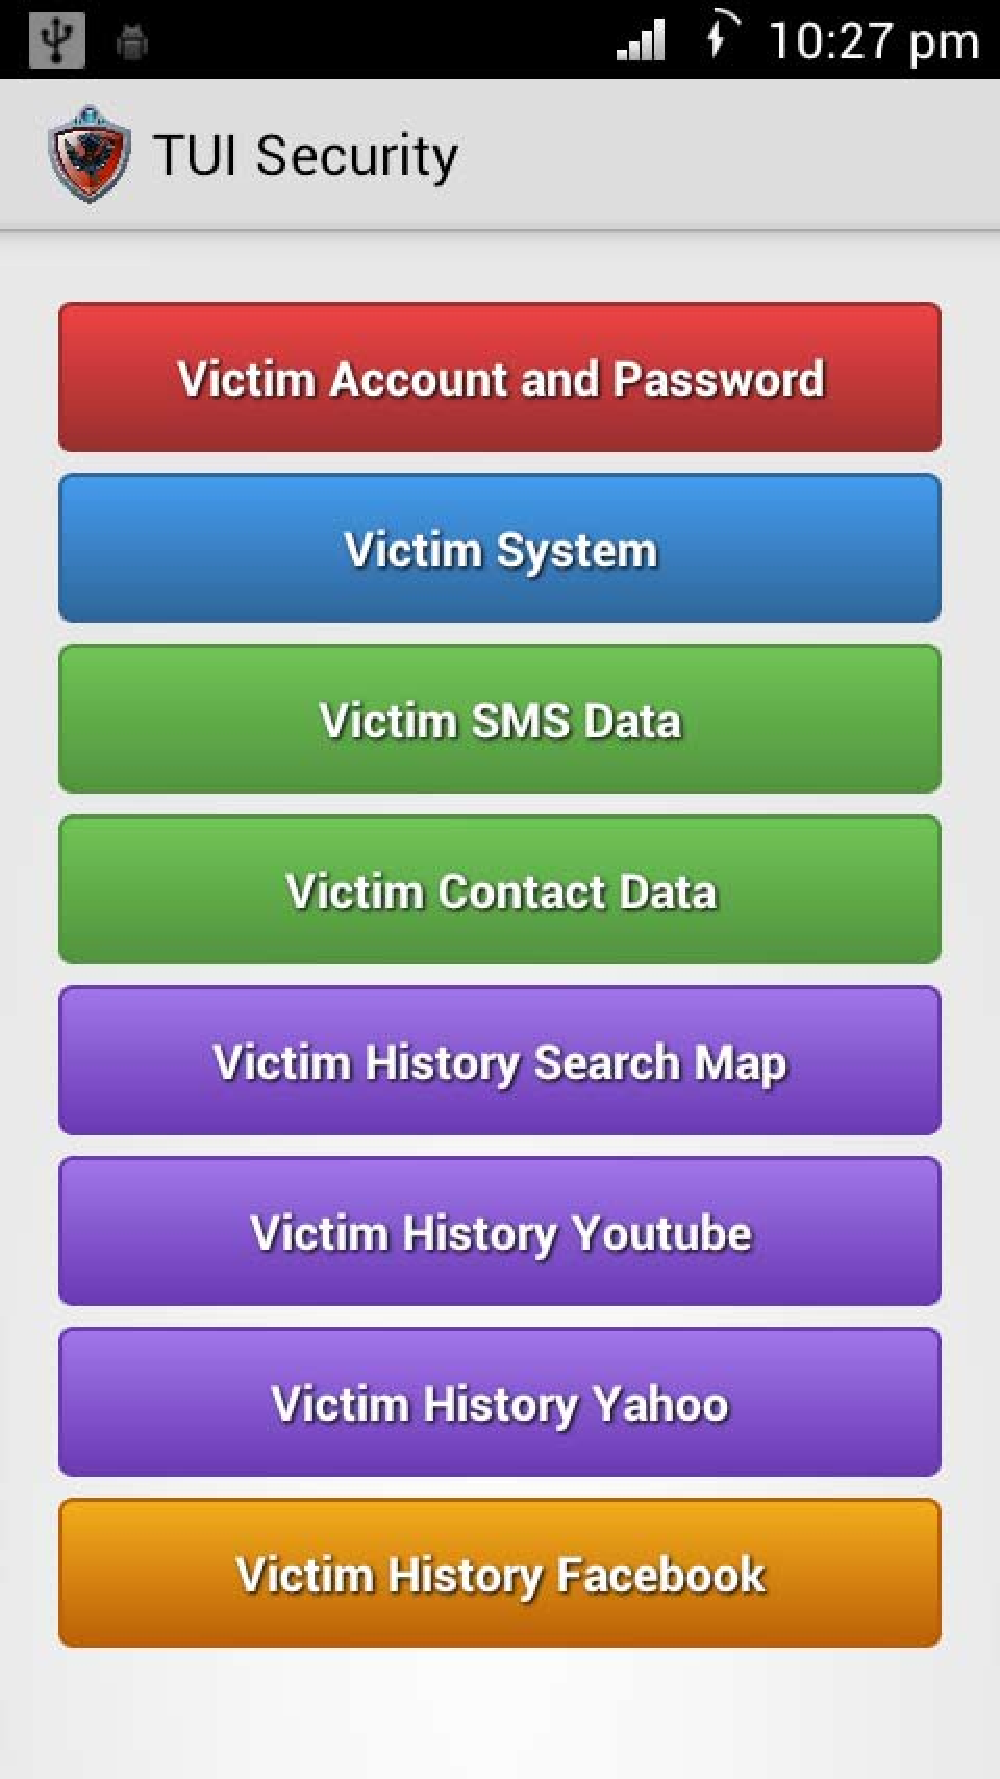
\includegraphics[width=0.30\textwidth] {tui-controls.pdf}
   \label{fig:tui-controls}}
\subfigure[tui-get-phone-info-controls]{
   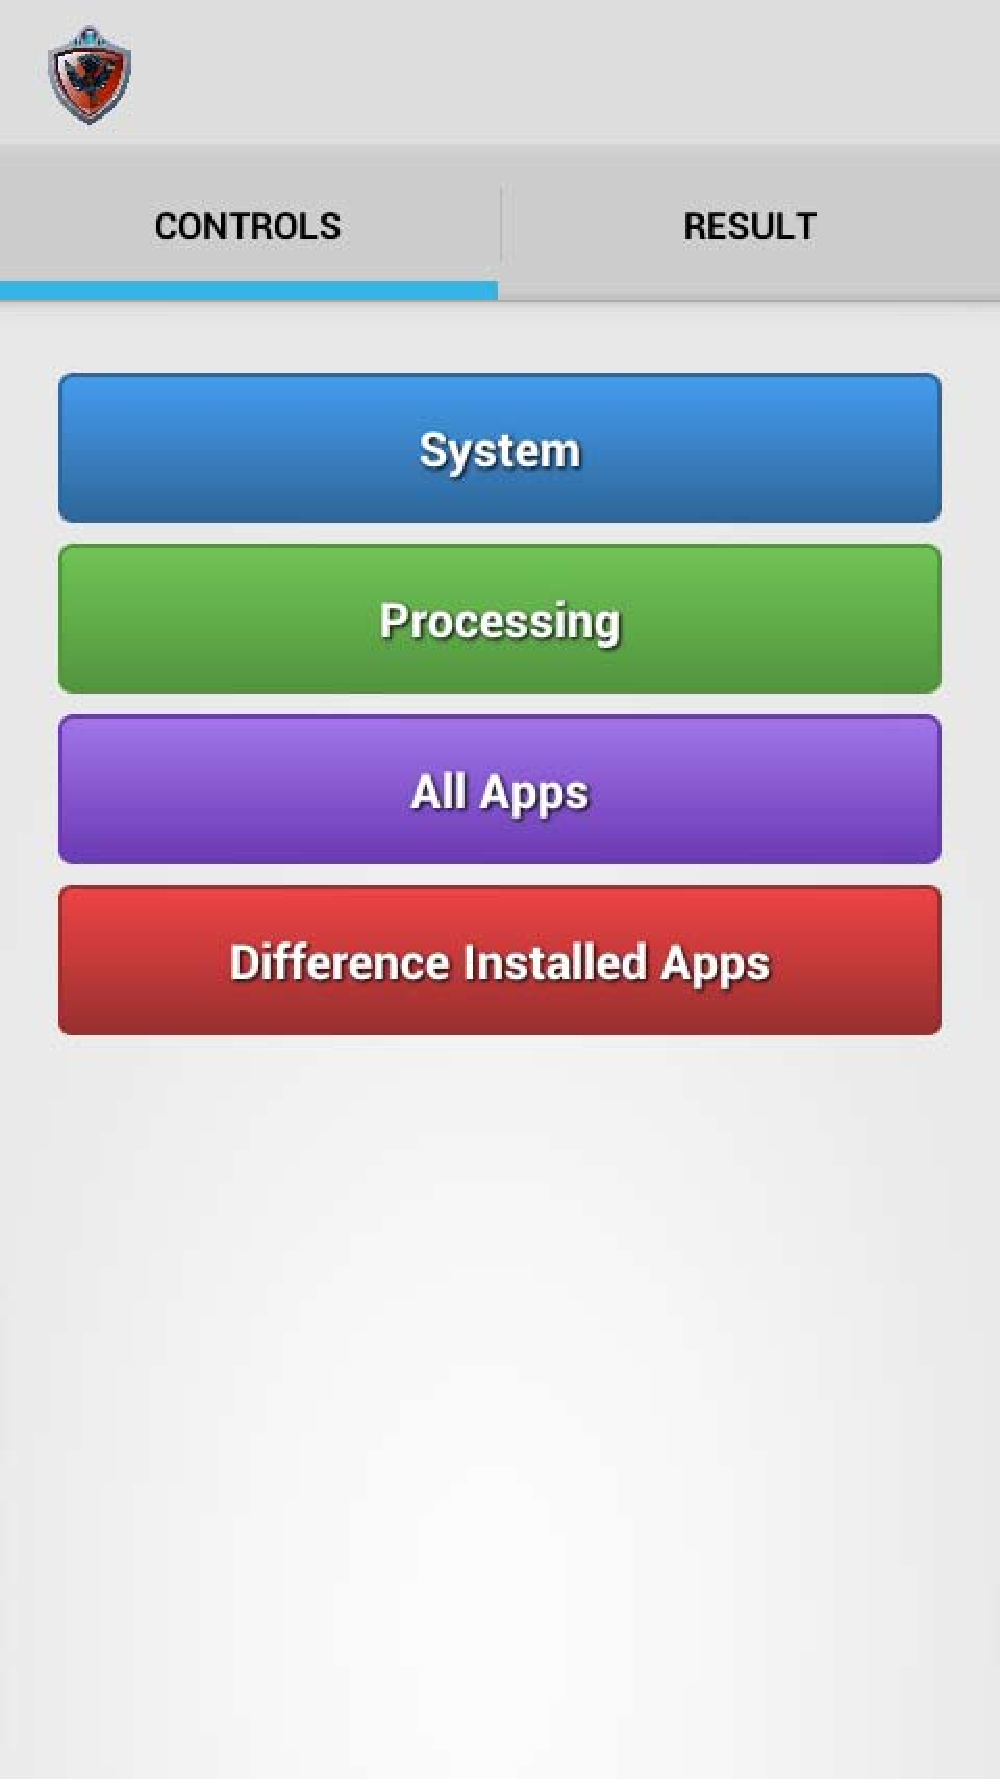
\includegraphics[width=0.30\textwidth] {tui-get-phone-info-controls.pdf}
   \label{fig:tui-get-phone-info-controls}}
\label{myfigure}
\caption{TUI security program main features}
\end{figure}

Viết luận văn bằng  \hologo{LaTeX}. Viết luận văn bằng  \hologo{LaTeX}. Viết luận văn bằng  \hologo{LaTeX}. Viết luận văn bằng  \hologo{LaTeX}. Viết luận văn bằng  \hologo{LaTeX}. Viết luận văn bằng  \hologo{LaTeX}. Viết luận văn bằng  \hologo{LaTeX}. Viết luận văn bằng  \hologo{LaTeX}. Viết luận văn bằng  \hologo{LaTeX}. Viết luận văn bằng  \hologo{LaTeX}. Viết luận văn bằng  \hologo{LaTeX}. Viết luận văn bằng  \hologo{LaTeX}. Viết luận văn bằng  \hologo{LaTeX}. Viết luận văn bằng  \hologo{LaTeX}. Viết luận văn bằng  \hologo{LaTeX}. Viết luận văn bằng  \hologo{LaTeX}. Viết luận văn bằng  \hologo{LaTeX}. Viết luận văn bằng  \hologo{LaTeX}. Viết luận văn bằng  \hologo{LaTeX}. Viết luận văn bằng  \hologo{LaTeX}. Viết luận văn bằng  \hologo{LaTeX}. 

Viết luận văn bằng  \hologo{LaTeX}. Viết luận văn bằng  \hologo{LaTeX}. Viết luận văn bằng  \hologo{LaTeX}. Viết luận văn bằng  \hologo{LaTeX}. Viết luận văn bằng  \hologo{LaTeX}. Viết luận văn bằng  \hologo{LaTeX}. Viết luận văn bằng  \hologo{LaTeX}. Viết luận văn bằng  \hologo{LaTeX}. Viết luận văn bằng  \hologo{LaTeX}. Viết luận văn bằng  \hologo{LaTeX}. Viết luận văn bằng  \hologo{LaTeX}. Viết luận văn bằng  \hologo{LaTeX}. Viết luận văn bằng  \hologo{LaTeX}. Viết luận văn bằng  \hologo{LaTeX}. Viết luận văn bằng  \hologo{LaTeX}. Viết luận văn bằng  \hologo{LaTeX}. Viết luận văn bằng  \hologo{LaTeX}. Viết luận văn bằng  \hologo{LaTeX}. Viết luận văn bằng  \hologo{LaTeX}. Viết luận văn bằng  \hologo{LaTeX}. Viết luận văn bằng  \hologo{LaTeX}. 


 
\subsubsection{first subsub section in the third subsection}
... and some more in the first subsub section otherwise it all looks the same
doesn't it? well we can add some text to it and some more and some more and
some more and some more and some more and some more and some more ...

\subsubsection{second subsub section in the third subsection}
... and some more in the first subsub section otherwise it all looks the same
doesn't it? well we can add some text to it ...

\section{Second Section of the Third Chapter}
\markboth{\MakeUppercase{\thechapter. My Third Chapter }}{\thechapter. My Third Chapter}
and here I write more ...


\section{Kết chương}
Viết luận văn bằng  \hologo{LaTeX}. Viết luận văn bằng  \hologo{LaTeX}. Viết luận văn bằng  \hologo{LaTeX}. Viết luận văn bằng  \hologo{LaTeX}. Viết luận văn bằng  \hologo{LaTeX}. Viết luận văn bằng  \hologo{LaTeX}. Viết luận văn bằng  \hologo{LaTeX}. Viết luận văn bằng  \hologo{LaTeX}. Viết luận văn bằng  \hologo{LaTeX}. Viết luận văn bằng  \hologo{LaTeX}. Viết luận văn bằng  \hologo{LaTeX}. Viết luận văn bằng  \hologo{LaTeX}. Viết luận văn bằng  \hologo{LaTeX}. Viết luận văn bằng  \hologo{LaTeX}. Viết luận văn bằng  \hologo{LaTeX}. Viết luận văn bằng  \hologo{LaTeX}. Viết luận văn bằng  \hologo{LaTeX}. Viết luận văn bằng  \hologo{LaTeX}. Viết luận văn bằng  \hologo{LaTeX}. Viết luận văn bằng  \hologo{LaTeX}. Viết luận văn bằng  \hologo{LaTeX}.  

